
%%%%%%%%%%%%%%%%%%%%%%%%%%%%%%%%%%%%%%%%%%%%%%%%%%%%%%%
% Section
%%%%%%%%%%%%%%%%%%%%%%%%%%%%%%%%%%%%%%%%%%%%%%%%%%%%%%%
\section{Collision Handling}\label{sec:collHandling}

Modeling and simulating the collisions between geometrical objects is difficult and there are many
methods dedicated to particular purposes. For example, in a game it is important that  
collisions of \emph{many} objects are supported in \emph{real-time} and that a simulation looks 
reasonably realistic. Game engines typically make compromises regarding physics (see for
example \cite{Erez2015}, where it is pointed out that NVIDIA PhysX and Havok neglect
Coriolis forces).
When designing an industrial product, it is important that collision models can be \emph{validated by measurements}. Therefore, the simulation results must
be much closer to reality as in a game.



\subsection{User's View}

Objects only take part in collision handling, if a \texttt{contactMaterial} is
associated with them. Modia3D uses two sets of material data:

\begin{enumerate}
\item \emph{Solid material constants}\\
      In a dictionary, the name of \emph{one} material is used as a key, for example \texttt{Steel}. 
      The values are typical material constants of a solid. For elastic response calculation,
      Young's modules $E$ and Poisson's ratio $\nu$ are used. From this data of two contacting
      objects, a spring constant is computed to describe the elastic deformation in the contact area.

\item \emph{Contact pair material constants}\\
      In another dictionary, the names of \emph{two} materials are used as a key, for example \texttt{Steel} 
      and \texttt{DryWood}. The values are the coefficient of restitution $cor$, 
      the kinetic/sliding friction force coefficient $\mu_k$ and the 
      rotational resistance torque coefficient $\mu_r$ between these two contacting
      objects of the respective materials, see section~\ref{sec:responseCalculation}.
\end{enumerate}  

A simple example is shown in Fig.~\ref{fig:bouncingBall}, where a
steel ball is bouncing on a wooden table.
This model is defined with the following Julia program
(\texttt{r} is the position vector from the parent -- defined with the first
argument -- to the reference frame of the object and \texttt{fixed} defines
whether the object is fixed or not fixed in space):
\newpage

\begin{lstlisting}[language = Julia]
@assembly BouncingBall begin
  world = Object3D()
  ball  = Object3D(world, Solid(SolidSphere(0.02),
		     ...;contactMaterial = "Steel");
		     r=[0,0,1.01], fixed=false)
  table = Object3D(world, Solid(SolidBox(1,1,0.1),
		     ...;contactMaterial = "DryWood"); 
		     fixed=true)
end

bounce = BouncingBall(sceneOptions=
          SceneOptions(enableContactDetection=true))
model  = SimulationModel(bounce)
result = simulate!(model; stopTime=3.0)
\end{lstlisting}


%
\begin{figure}[tb]
	\centering
	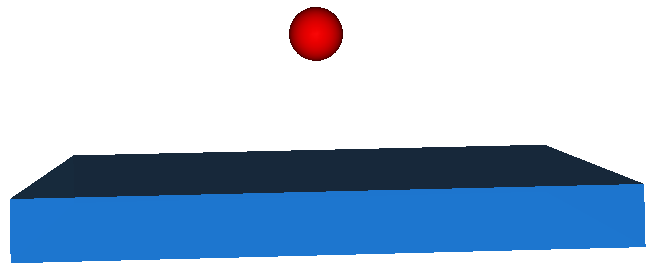
\includegraphics[width=0.2\textwidth]{figures/bouncingBall.png}
	\caption{Ball falling on a table.}
	\label{fig:bouncingBall}
\end{figure}
%
During simulation, the \texttt{contactMaterials} defined for
\texttt{ball} and for \texttt{table} are used as keys in the two
dictionaries sketched above. 
When the two objects penetrate each other,
an elastic response is computed with the help of the dictionary values 
(provided collision handling was explicitly enabled in the scene options).

\subsection{Numerical Solution}\label{sec:numericSolution}

\newcommand{\bvec}[1]{\bm{#1}}

A Modia3D model is mathematically defined by the hybrid DAE system~(\ref{eq:DAE}), 
where $\bvec{x} = \bvec{x}(t)$ 
and $\bvec{J}$ (\ref{eq:DAE}c) is a \emph{regular} Jacobian:
%
\begin{equation} \label{eq:DAE}
\begin{aligned}
\bvec{0} = & \; \left[\begin{aligned}
& \bvec{f}_d(\dot{\bvec{x}},\bvec{x},t, z_i > 0) \\
& \bvec{f}_c(\bvec{x},t, z_i > 0)
\end{aligned}\right]  & (a) \\
\bvec{z} = & \; \bvec{f}_z(\bvec{x},t) & (b)
\end{aligned} \quad
\bvec{J} = \left[\begin{aligned}
& \frac{\partial\bvec{f}_d}{\partial\dot{\bvec{x}}} \\
& \frac{\partial\bvec{f}_c}{\partial{\bvec{x}}}
\end{aligned}\right] \; (c)
\end{equation}
%
When differentiating $\bvec{f}_c$ once, it is (conceptually) possible to
solve (\ref{eq:DAE}c) for $\dot{\bvec{x}}$ because $\bvec{J}$ is regular.
Therefore, (\ref{eq:DAE}a) is an index 1 DAE. (\ref{eq:DAE}b) defines zero-crossing functions $\bvec{z}(t)$. 
Whenever a $z_i$ crosses zero, an event is triggered, simulation is halted, functions
$\bvec{f}_d, \bvec{f}_c$ can be changed, and simulation is restarted. 
(\ref{eq:DAE}) is numerically solved with the variable-step
DAE integrator IDA of the Sundials suite~\cite{Sundials2005} via the
Sundials.jl~\cite{Rackauckas2017} Julia package. Since contact forces and torque
lead to extreme changes of $\bvec{f}_d, \bvec{f}_c$, 
the distances between convex shapes are used as zero-crossing functions $z_i(t)$ so
that the start and the end of a contact phase triggers an event. It is expected that this
approach improves the reliability of a simulation. Furthermore, the elastic response
calculation of section \ref{sec:responseCalculation} needs the relative velocity 
when a contact starts, to compute an appropriate 
damping factor $d$. Therefore, an event at the start of a contact is mandatory.

Distances between convex shapes, as well as penetration depths are computed with an improved version of the
Minkowski Portal Refinement algorithm (MPR-algorithm) \cite{snethen2008}.
The MPR-algorithm is much simpler to implement and has less numerical problems than the often used GJK/EPA-standard algorithms \cite{bergen2003, GJK1988}, because it only works with triangles and not with tetrahedrons.
In the original version of the MPR-algorithm \cite{snethen2008} only penetration depths are determined. In Modia3D improvements of the MPR-algorithm are utilized that have been proposed in \cite{kenwright2015,Neumayr2017}, in particular to compute the distances of shapes that are not in contact
and treat special collision situations properly.

Collisions of $n$ potentially colliding shapes are handled in the following (mostly standard) way:
\begin{enumerate}
	\item[1. ] \emph{Broad Phase}\\
	The shapes are approximated by \emph{Axis Aligned Bounding Boxes}, see e.g.\ \cite{bergen2003},
    where potential collisions and approximate distances can be very cheaply determined
	resulting in $O(n^2)$ cheap tests. When using special data structures (such as octrees or kd-trees),
	it is even possible to reduce the number of cheap tests to $O(n \log(n))$.
	
	\item[2. ] \emph{Narrow Phase}\\
	For the potentially colliding shape pairs as identified in the broad phase,
	the signed distances are computed with the improved MPR-algorithm \cite{Neumayr2017}.
	
	\item[3. ] \emph{Response Calculation} \\
	If two shapes are penetrating, a normal and a tangential force, as well as a torque are applied at the
	contact point. For details, see section \ref{sec:responseCalculation} and 
    Fig.~\ref{fig:forces}.
\end{enumerate}


\subsection{Elastic Response Calculation}\label{sec:responseCalculation}

A contact normal force $\vec{f}_n$, a contact tangential force $\vec{f}_t$ (= sliding friction force), 
and a contact torque $\vec{\tau}_{\omega}$ are calculated when two 3D objects penetrate each other with a 
penetration depth $\delta \ge 0$, as shown in Fig.~\ref{fig:forces}. The intuition is that
there is a contact area with a certain pressure distribution in normal and a stress
distribution in tangential direction and that the response characteristics provides an
approximation of the resultant force and torque of these distributions.
%

\begin{figure}[t]
	\centering
	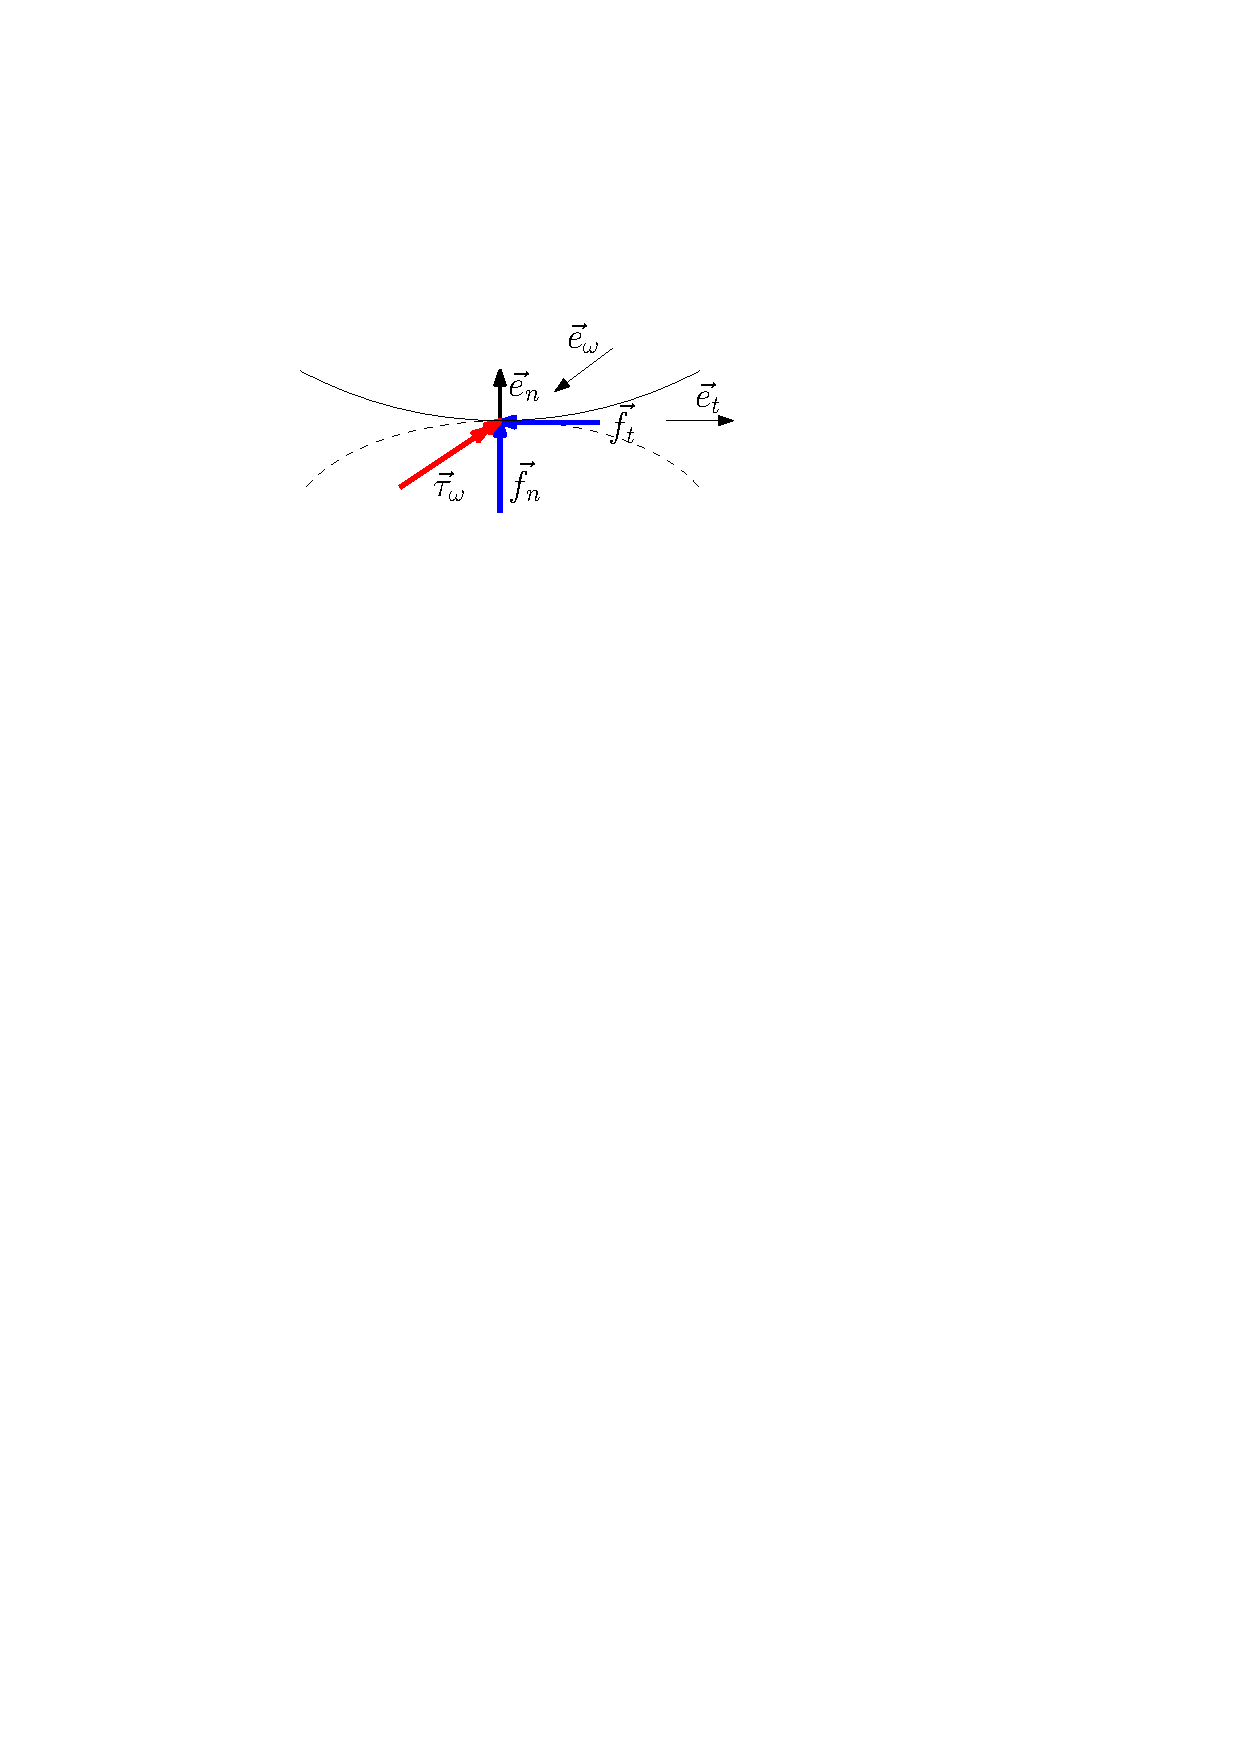
\includegraphics[width=0.25\textwidth]{figures/forces.pdf}
	\caption{Contact normal force $\vec{f}_n$, contact tangential force $\vec{f}_t$ 
		(= sliding friction force) and contact torque $\vec{\tau}_{\omega}$
		between two penetrating objects. $\vec{e}_n, \vec{e}_t, \vec{e}_{\omega}$ are unit vectors
		in direction of the respective relative movement.}
	\label{fig:forces}
\end{figure}

%
The MPR-algorithm computes the contact point, $\delta$, and a unit vector $\vec{e}_n$ that is orthogonal
to the contacting surfaces. The novel response characteristic of (\ref{eq:response})
utilizes ideas from \cite{Flores2011, otter2005, Skinjar2018} with some extensions
and corrections. Variables with index ${geo}$ are computed from the contacting geometries and 
vectors with index ${reg}$ are regularized with smooth characteristics  to avoid divisions by zero
(for example, $|\vec{e}_{t,reg}| = 1$ with exception of a small region around
$|\vec{v}_{rel,t}| < v_{small}$, where $|\vec{e}_{t,reg}| = 0$ at
$|\vec{v}_{rel,t}| = 0$ and it smoothly approaches $1$ at $|\vec{v}_{rel,t}| = v_{small}$):
%
\begin{subequations}
\begin{align}
f_n 	  & = max \biggl( 0, c_{res} \, c_{geo} \, \delta^{n_{geo}} \Bigl( 1 + d \, \dot{\delta} \Bigl) \biggl) \\
\vec{f}_n & = f_n \vec{e}_n \\
\vec{f}_t & = - \mu_k f_n \vec{e}_{t,reg} \\
\vec{\tau}_{\omega} & = - \mu_r \mu_{geo} f_n \vec{e}_{\omega, reg}
\end{align}
\label{eq:response}
\end{subequations}
%
The symbols of (\ref{eq:response}) have the following meaning:

\begin{description}[labelwidth=3ex]
\item[$\vec{e}_n$] Unit vector normal to the contacting surfaces.
\item[$\vec{e}_t$] Unit vector in direction of the relative tangential velocity.
\item[$\vec{e}_{\omega}$] Unit vector in direction of the relative angular velocity.
\item[$c_{res}(E_1, E_2, \nu_1, \nu_2)$]  Resultant spring constant in normal direction.
                   $c_{res}=1/(1/c_1+1/c_2); \; c_i=E_i/(1 - \nu_i^2$). 

\item[$d(cor_{reg}, \dot{\delta}^{-})$] Damping coefficient as function of the regularized
                   coefficient of restitution $cor_{reg}$ and $\dot{\delta}$
                   when contact starts ($\dot{\delta}^{-} \ge 0$).
                   Variable $cor_{reg}$ is computed according to \cite{Flores2011} and regularized
                   so that $cor_{reg} = 0.001$ if the normal relative velocity $v_{rel,n}=\SI{0}{\meter \per \second}$
                   and approaches $cor$ when $v_{rel,n} = v_{small}$.
                   One reason for this is
                   that otherwise \cite{Flores2011} would result in a division by zero if 
                    $cor =  0$. The other reason is that a bouncing object stays at rest if 
                   $v_{rel,n}$ becomes small enough and therefore $cor_{reg}$ must be drastically
                   reduced for small $v_{rel,n}$ (this effect is typically not taken
                   into account in other contact laws, such as in \cite{Skinjar2018}).
\item[$\mu_k$]     Kinetic/sliding friction force coefficient ($\ge 0$).
\item[$\mu_r$]     Rotational resistance torque coefficient ($\ge 0$). 
                   Its effect is that torque $\vec{\tau}_{\omega}$ is computed to reduce the relative
                   angular velocity $\vec{\omega}_{rel}$ between the two objects until $\vec{\omega}_{rel}= \SI{0}{\radian\per\second}$.
                   For a ball, $\mu_r$ is the (standard) rolling resistance coefficient and
                   $\mu_{geo}$ is the ball radius.
\end{description}
%
$c_{geo}, n_{geo}, \mu_{geo}$ depend on the geometries of the two objects in contact.
If not enough information is available, these factors are set to one.
$c_{geo}, n_{geo}$ take the contact volume into account, under the assumption of Hertz' pressure (e.g.\ $n_{geo} = 3/2$ if at least one of the
two contacting objects is a sphere).

The response characteristics (\ref{eq:response}) shall be clarified with a few special
experiments:

\subsubsection*{Comparison between elastic and impulsive contact response}

In Fig.~\ref{fig:bouncingBallPlot}, the height of the bouncing ball (see model
of Fig.~\ref{fig:bouncingBall}) is shown as a function of time.
%
\begin{figure}[b]
	\centering
	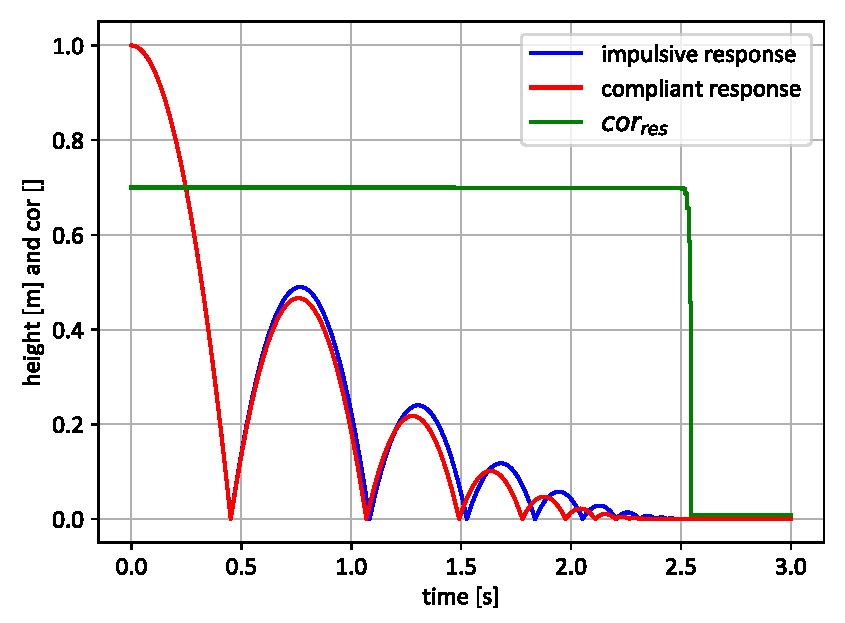
\includegraphics[width=0.48\textwidth]{figures/bouncingBall_plot.pdf}
	\caption{Bouncing ball (see Fig.~\ref{fig:bouncingBall}) with impulsive contact
             and the elastic response characteristic of (\ref{eq:response}).}
	\label{fig:bouncingBallPlot}
\end{figure}
%
The red curve is the reaction when using the elastic response calculation of 
(\ref{eq:response}) with $cor = 0.7$ and the solid material constants of steel and of
dry wood. The blue curve is the result when
the contact force is computed with an impulse for the same $cor$ value.
The green curve is $cor_{reg}$ (for small velocities it becomes small).
This shows that $f_n$ in (\ref{eq:response}) leads to a similar reaction if
compared to an impulsive response. Note, this was the intention for the development
of this force law in \cite{Flores2011}. A systematic comparison was made in \cite{Skinjar2018}.
 
\subsubsection*{Sliding and rolling ball}

In Fig.~\ref{fig:rollingBall} an animation of a billiard ball is shown that is sliding and rolling
on a billiard table. 
%
\begin{figure}[bt]
	\centering
	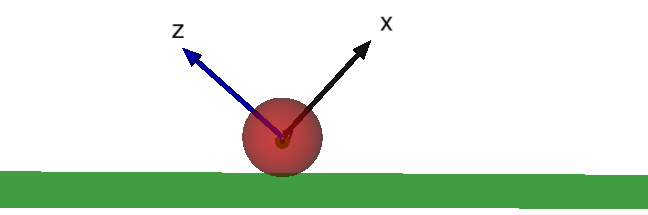
\includegraphics[width=0.3\textwidth]{figures/rollingBall.png}
	\caption{Billiard ball sliding and rolling on a billiard table.}
	\label{fig:rollingBall}
\end{figure}
%
The billiard ball is a free flying object with 6 degrees-of-freedom where the rotation is
described with quaternions (in total, the state of this object is defined with 13 variables). 
It starts at its initial position $r_s = \SI{0.2}{\meter}$ with an initial velocity $v_s = \SI{3}{\meter \per \second}$ . At initialization, the billiard ball is placed in touching position with the table (penetration depth $\delta = 0$). The ball subsides immediately, because of gravity in z-direction. Therefore, the ball and the table are colliding, a collision event is triggered, and the two objects are penetrating each other. The material data is shown in table \ref{table:billiardTableMaterials}.

%
\begin{figure}[tb]
	\centering
	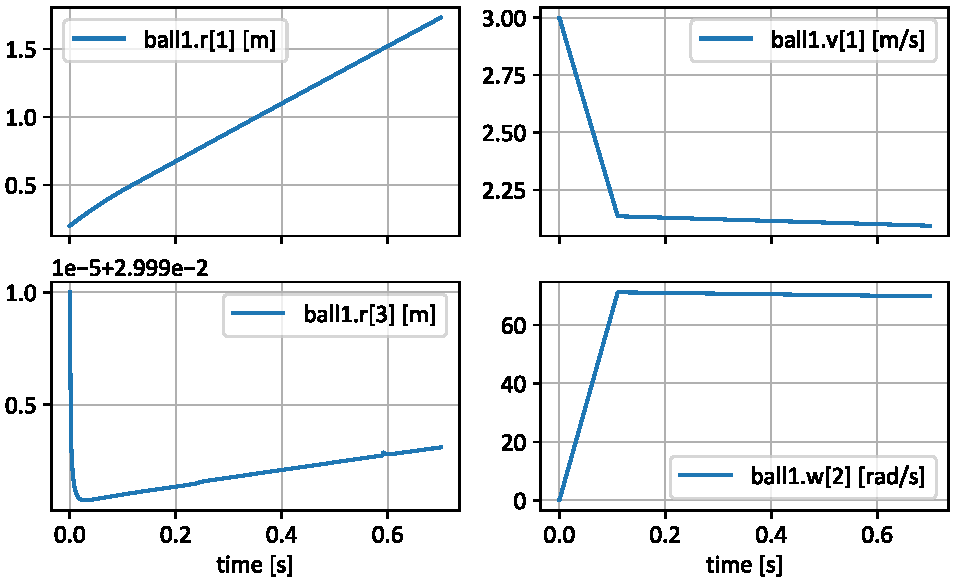
\includegraphics[width=0.47\textwidth]{figures/rollingBall_plot.pdf}
	\caption{Position of a sliding and rolling billiard ball in x- and z-direction, velocity in x-direction, and angular velocity in y-direction.}
	\label{fig:rollingBall_plot}
\end{figure}
%
The upper left plot in Fig,~\ref{fig:rollingBall_plot} shows the position of the billiard ball in x-direction. 
The lower left plot of Fig.~\ref{fig:rollingBall_plot} shows the subsidence of the ball into the table 
which is in the order of $10^{-5}$ m. The upper right plot shows the velocity of the ball in 
x-direction and the lower right plot displays the angular velocity in y-direction.
The first $\SI{0.15}{\second}$ the ball is sliding. Due to sliding friction ($\mu_k = 0.6$), the relative velocity is reduced.
At the same time, the sliding friction force acts as a torque around the ball center and forces a rotation of
the ball around the y-direction. At $time = \SI{0.15}{\second}$, the relative velocity in tangential direction $v_{rel,t}$ is zero 
\begin{equation}
v_{rel,t} = v_{ball,1} - \omega_{ball,2} r_{ball} = 2.125 - 70 \cdot 0.03 \approx \SI{0}{\meter \per \second}
\end{equation}
and \emph{ideal rolling} of the ball takes place. Since $v_{rel,t} =\SI{0}{\meter \per \second}$, the sliding friction force
$\vec{f}_t = \SI{0}{\newton}$, because $\vec{e}_{t,reg}= 0$. Therefore, the ball would roll forever, contrary to reality.
On the other hand, the rotational resistance torque $\vec{\tau}_{\omega}$ ($\mu_r = 0.02$) acts as a
rolling resistance that continuously reduces the
angular velocity $\omega_{ball,2}$ and the ball comes to rest at 
some point in the future outside of the plot area (see right upper and lower plot of 
Fig.~\ref{fig:rollingBall_plot}). The result is that
(\ref{eq:response}) is able to reproduce the effect of a sliding and rolling 
ball. However, for simplicity of the formulation, in this simplistic elastic
response law, velocity dependency of the coefficients $cor, \mu_k, \mu_r$ is neglected.


\subsubsection*{Collision of two balls}

Two billiard balls are positioned on a billiard table, see Fig.~\ref{fig:twoCollidingBalls}.
One of them has an initial velocity and hits the other resting ball after some time.
Simulation results are shown in Fig.~\ref{fig:twoCollidingBalls_plot}.
Before the first ball hits the second one, the
effects of sliding and rolling occur as analyzed before.
%
\begin{figure}[b]
	\centering
	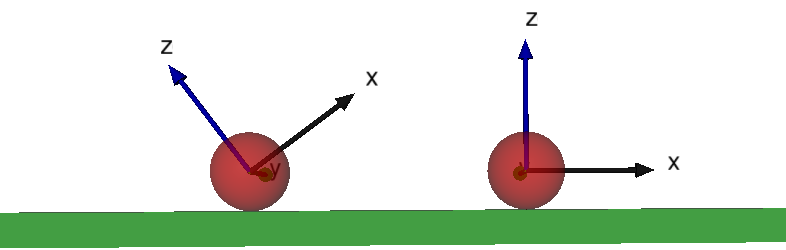
\includegraphics[width=0.35\textwidth]{figures/twoCollidingBalls.png}
	\caption{Billiard ball colliding with another billiard ball.}
	\label{fig:twoCollidingBalls}
\end{figure}
%
\begin{figure}[t]
	\centering
	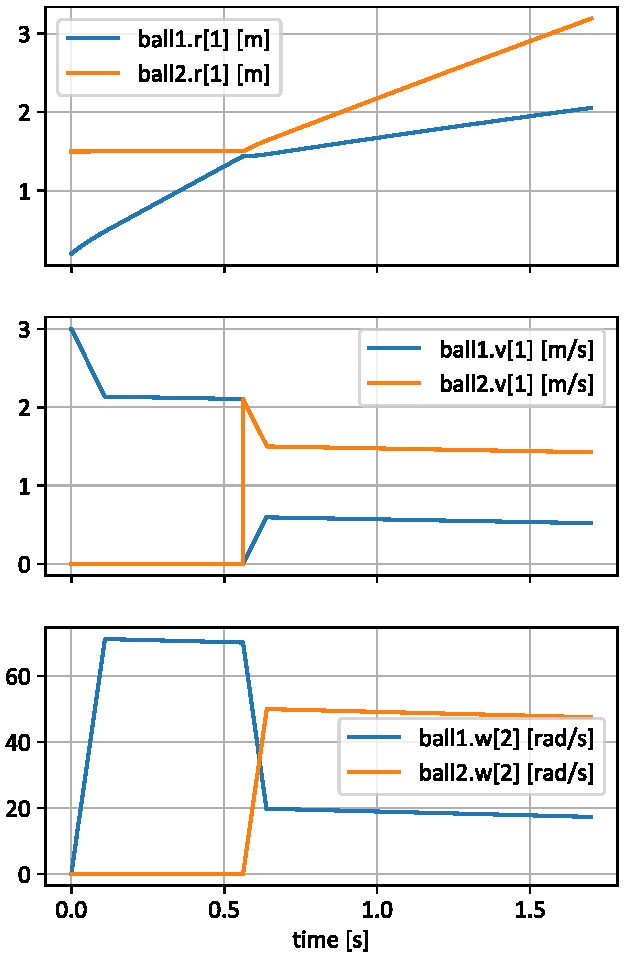
\includegraphics[width=0.35\textwidth]{figures/twoCollidingBalls_plot.pdf}
	\caption{Position of two colliding billiard balls, velocity in x-direction, and angular velocity in y-direction.}
	\label{fig:twoCollidingBalls_plot}
\end{figure}
%
At $time = \SI{0.55}{\second}$, the first ball hits the second ball. Since the coefficient of restitution between the
two balls is one, a fully elastic collision takes place. In this case the first ball transfers most of its kinetic energy to the second ball which starts moving with the velocity of the first ball. This ``exchange`` of velocity
can be observed in the middle plot of Fig.~\ref{fig:twoCollidingBalls_plot} at $time = \SI{0.55}{\second}$. However, since the first ball
was rolling, the angular momentum was greater zero. This momentum is conserved. Therefore, the first ball continues rolling
and velocity $v_{ball,1}$ rises from zero again.
Since the relative velocity is no longer zero due to the impact, again a friction force $\vec{f}_t$ is acting
that introduces a counter torque at the balls axis which quickly reduces the angular velocity until again
the relative velocity is zero around $time = \SI{0.65}{\second}$. Both balls are again ideally rolling, and due to the
rotational resistance torque, the angular velocities are slowly reduced until both balls come to rest
which is not shown in the plots.
%



\subsection{Regularizing the Contact Area}\label{sec:BouncingBox}

A DAE solver such as IDA, see Section \ref{sec:numericSolution}, solves a nonlinear algebraic
equation system at every time instant. If $\bvec{f}_d, \bvec{f}_c$ in (\ref{eq:DAE}) are not smooth or even not continuous,
it is most likely that no solution of this algebraic equation system is found and simulation stops.
This situation occurs easily, for example, if the edges or vertices of two boxes collide on each other, because very small changes of the
positions of the boxes can change the contact situation drastically. To improve the reliability of the simulation, Modia3D
uses the approach proposed in \cite{bergen2003}, and is smoothing every shape with a small sphere (default radius $= \SI{1}{\milli \meter}$) that
is (conceptually) moved over all surfaces. Practically, this smoothing can be very easily and cheaply incorporated for the
convex collision handling. 

Every method that considers only contact points on two colliding objects and the corresponding penetration depth has the
disadvantage that an infinite number of solutions can occur in some cases. For example this happens, when a box falls on a table and the faces of box and table are parallel. Imagine small changes in the configuration can result in identification of very different contact points in the contact area.
It is then highly probable that simulation with a variable-step solver fails. Furthermore, the contact force and torque
depend heavily on the size of the contact area. The penetration depth alone does not provide enough information
to calculate reasonable values that are in accordance with physics. For both cases, it would be necessary to take the
complete contact area and volume into account, as done e.g. in \cite{Elmqvist2015}. This method is however much more costly
and probably only works reasonably for soft contacts where the contact volume is large enough.
To summarize, collision handling with variable-step solvers and penetration depth computation 
can most likely only work reliably for point contacts that are smoothly changing.

